% Figure from MATH 591 notes, section 60. Compile with the notes preamble.
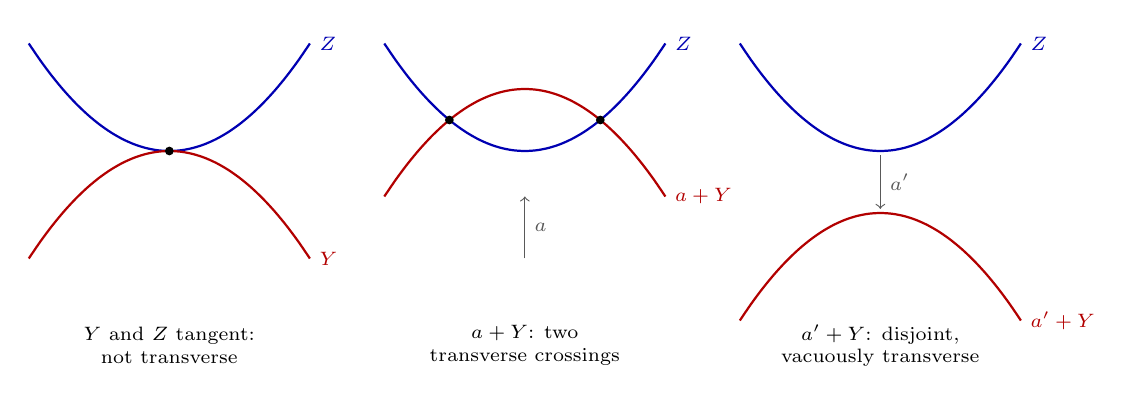
\begin{tikzpicture}[scale=1.05, font=\scriptsize]
\foreach \dx/\dy/\lab/\cap [count=\i] in {0/0/Y/{$Y$ and $Z$ tangent:\\ not transverse}, 4.3/0.75/{a+Y}/{$a + Y$: two\\ transverse crossings}, 8.6/-0.75/{a'+Y}/{$a' + Y$: disjoint,\\ vacuously transverse}} {
  \begin{scope}[xshift=\dx cm]
  \draw[blue!70!black, thick] plot[smooth, domain=-1.7:1.7] (\x,{0.45*\x*\x});
  \node[blue!70!black, anchor=west] at (1.7,1.3) {$Z$};
  \draw[red!70!black, thick] plot[smooth, domain=-1.7:1.7] (\x,{-0.45*\x*\x+\dy});
  \node[red!70!black, anchor=west] at (1.7,{-1.3+\dy}) {$\lab$};
  \node[align=center] at (0,-2.35) {\cap};
  \end{scope}}
\fill (0,0) circle (1.5pt);
\fill ({4.3-sqrt(0.75/0.9)},{0.45*0.75/0.9}) circle (1.5pt); \fill ({4.3+sqrt(0.75/0.9)},{0.45*0.75/0.9}) circle (1.5pt);
\draw[->, gray!70!black] (4.3,-1.3) -- node[right] {$a$} (4.3,-0.55);
\draw[->, gray!70!black] (8.6,-0.05) -- node[right] {$a'$} (8.6,-0.7);
\end{tikzpicture}
